\documentclass{article}
\usepackage{amsmath,amsfonts,amssymb,bm,mathtools,upgreek}
\usepackage{caption}
\usepackage{fancyhdr}
\usepackage{float}
\usepackage{fixmath}
\usepackage[T1]{fontenc}
\usepackage[margin=1in]{geometry}
\usepackage{graphicx}
\usepackage{hyperref}
\usepackage[utf8]{inputenc}
\usepackage{lipsum}
\usepackage{siunitx}
\usepackage{subcaption}
\usepackage{optidef}

\graphicspath{ {../figures/} }

\setlength{\parindent}{0pt}
\setlength{\parskip}{.5em}

\title{CS 5033: Final Project Report}
\author{Shane Flandermeyer}
\date{}

% TODO: Make the spacing look good
\begin{document}

\maketitle

\section{Introduction}

The rapid evolution of wireless communications technologies such as 4G/5G and the internet-of-things (IoT)
has radically altered daily life. These technologies utilize the radio frequency (RF) portion of the electro-
magnetic spectrum, which is a finite resource. To effectively access and regulate the spectrum, it is essential
that the next generation of wireless devices be able to rapidly classify and monitor signals in the spectrum.
Information gained from sensing the spectrum can be used for tasks such as cognitive radio, interference
detection, and dynamic spectrum access \cite{Kulin2018}. Signal
detection and classification has traditionally been accomplished through static filtering and
signal processing using expert features \cite{Ariananda2009}. However, a
data-adaptive approach is needed to improve spectrum efficiency to meet modern
wireless data demands.

For this project, I have developed a training and testing dataset generation
tool for RF signal classification networks. This tool follows the process outlined
in \cite{OShea2016}, which uses GNU Radio to simulate the effects of hardware
and propagation through a channel (e.g., free space). The tool is currently
capable of simulating six different types of signals (four
communications-based, two radar-based) and my object-oriented approach makes it
easily extensible to others. To verify the output of the tool, I have also
implemented a modified version of the convolutional neural network (CNN)
described in \cite{OShea2016a}.


\section{Methodology}

% Describe the technique you are working
% with e.g., if you are implementing/developing
% an algorithm, explain that algorithm
% mathematically.

\begin{figure}[H]
    \centering
    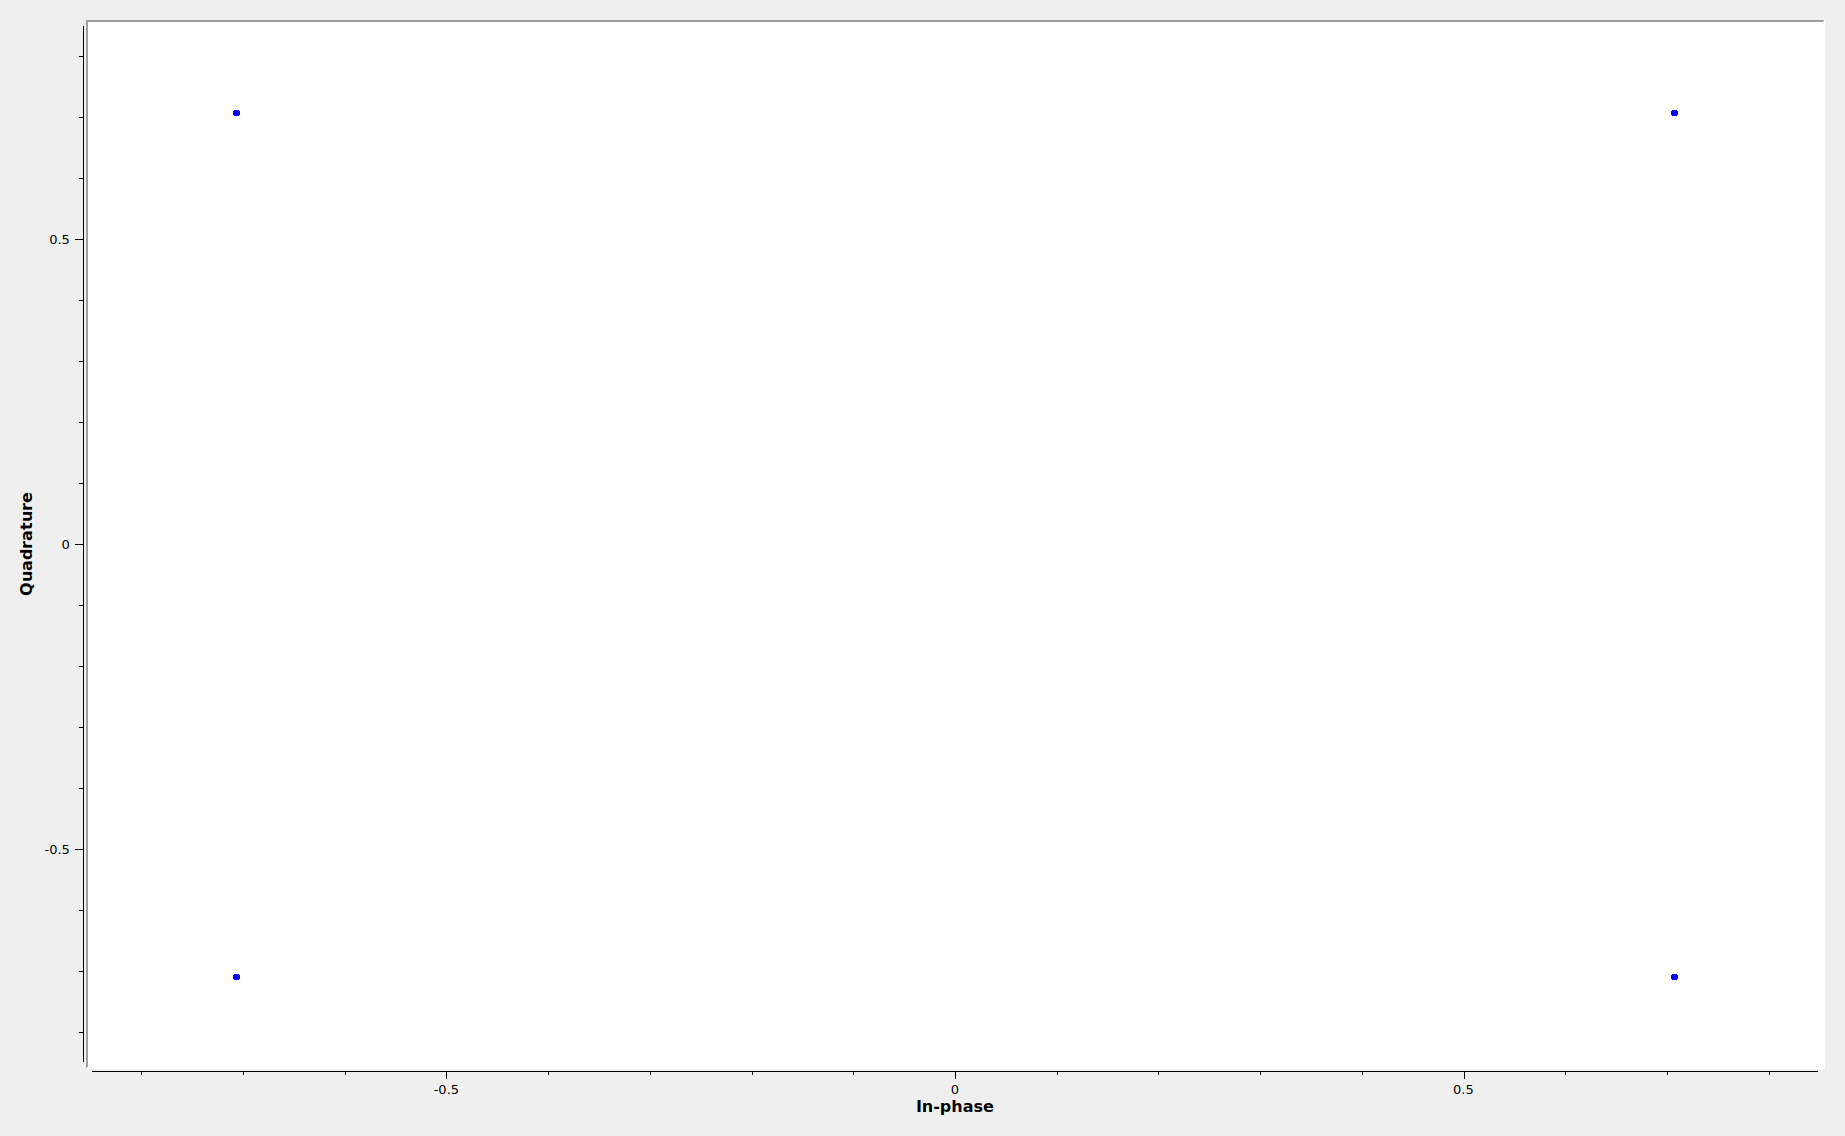
\includegraphics[width=0.45\linewidth]{qpsk.png}
    \caption{RRC-filtered QPSK signal}
    \label{fig:qpsk}
\end{figure}

\begin{figure*}
    \centering
    \begin{subfigure}[b]{0.475\textwidth}
        \centering
        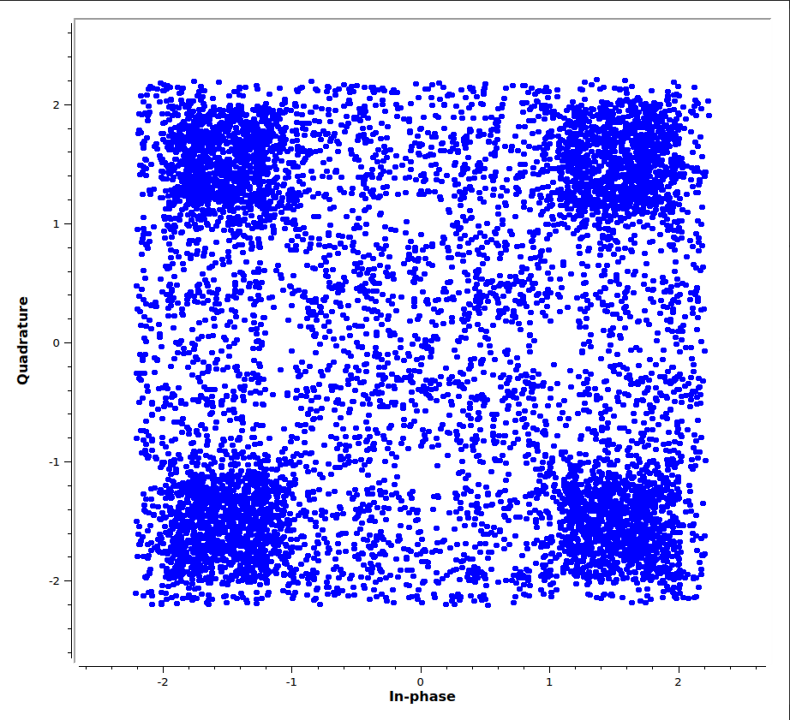
\includegraphics[width=\textwidth]{sro.png}
        \caption[]%
        {{\small Sample Rate Offset}}    
        \label{fig:sro}
    \end{subfigure}
    \hfill
    \begin{subfigure}[b]{0.475\textwidth}  
        \centering 
        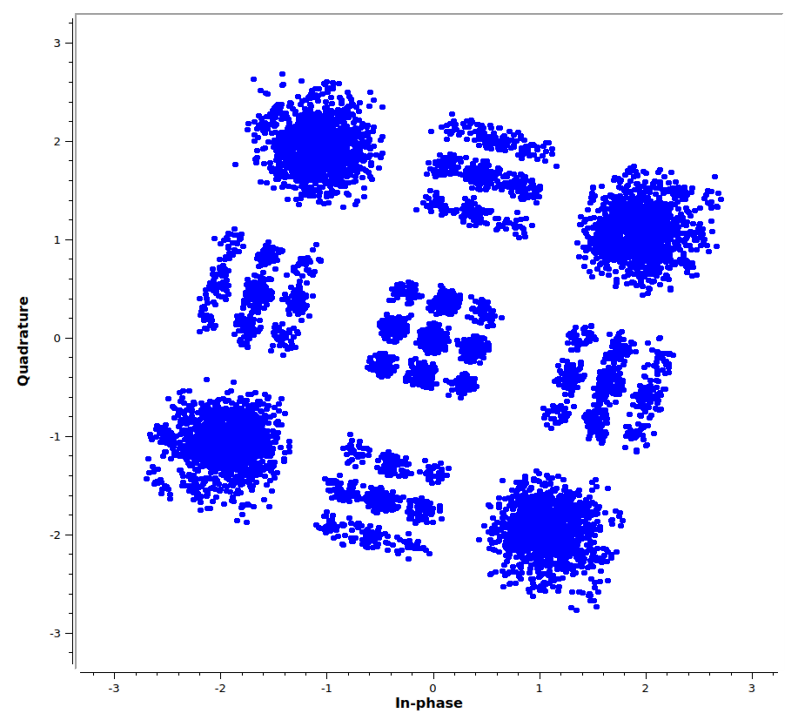
\includegraphics[width=\textwidth]{cfo.png}
        \caption[]%
        {{\small Center Frequency Offset }}    
        \label{fig:cfo}
    \end{subfigure}
    \vskip\baselineskip
    \begin{subfigure}[b]{0.475\textwidth}   
        \centering 
        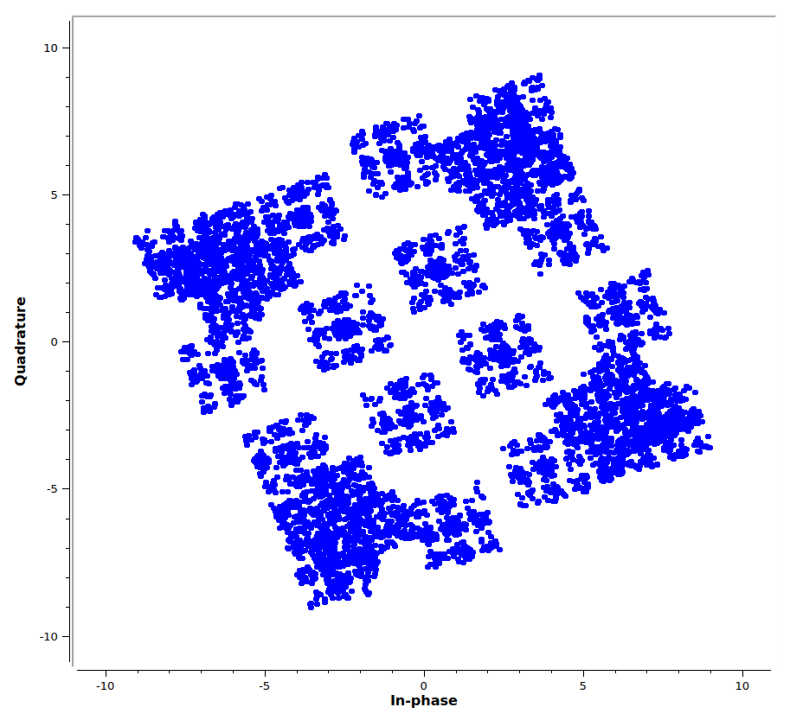
\includegraphics[width=\textwidth]{fading.png}
        \caption[]%
        {{\small Channel Fading}}    
        \label{fig:fading}
    \end{subfigure}
    \hfill
    \begin{subfigure}[b]{0.475\textwidth}   
        \centering 
        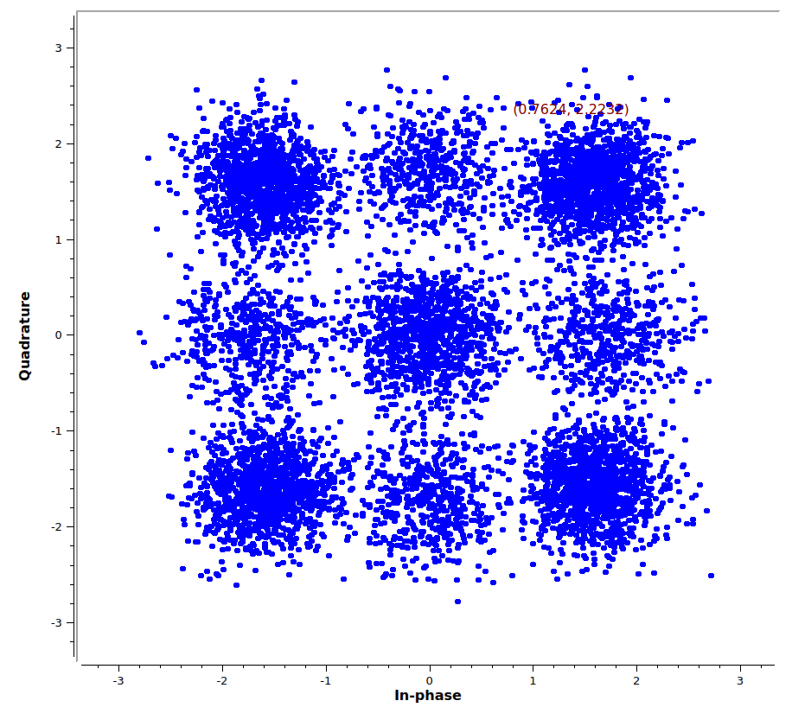
\includegraphics[width=\textwidth]{awgn.png}
        \caption[]%
        {{\small Additive White Gaussian Noise}}    
        \label{fig:awgn}
    \end{subfigure}
    \caption[]
    {} 
    \label{fig:channel model}
\end{figure*}

\section{Experiment}

\subsection{Data Preparation}

\begin{figure}[H]
    \centering
    \includegraphics[width=\linewidth]{waveforms.png}
    \caption{Waveforms used for Experiment}
    \label{fig:waveforms}
\end{figure}


Describe how you collected data, how
you cleaned the data (if you did).

\subsection{Experiment Design}

% TODO: Describe the simulation loop in synthesize_data

Describe how you design experiment,
e.g., how to split training data and testing
data; how to choose hyper-parameters; how
to evaluate model performance (accuracy/f1/AUC).

\subsection{Results and Discussion}

\begin{figure}[H]
    % TODO: Replace these placeholder figures
    \centering
    \begin{subfigure}[b]{0.3\textwidth}
        \centering
        \includegraphics[width=\textwidth]{waveforms.png}
        \caption{Noise Voltage = 20 dB}
        \label{fig:noise voltage = 20 dB}
    \end{subfigure}
    \hfill
    \begin{subfigure}[b]{0.3\textwidth}
        \centering
        \includegraphics[width=\textwidth]{waveforms.png}
        \caption{Noise Voltage = -$\infty$ dB}
        \label{fig:noise voltage = 0}
    \end{subfigure}
    \hfill
    \begin{subfigure}[b]{0.3\textwidth}
        \centering
        \includegraphics[width=\textwidth]{waveforms.png}
        \caption{Full Test Set}
        \label{fig:full test set}
    \end{subfigure}
       \caption{Confusion Matrices}
       \label{fig:confusion}
\end{figure}

\begin{figure}[H]
    \centering
    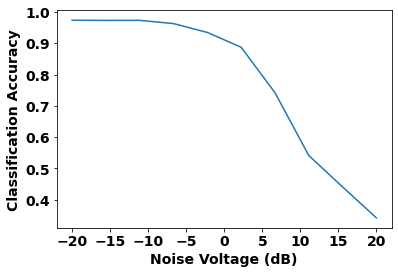
\includegraphics[width=0.45\linewidth]{classification-accuracy.png}
    \caption{Classification Accuracy vs SNR}
    \label{fig:classification accuracy}
\end{figure}

Present your experimental results and discuss
the results (e.g. what can we learn from the
results?)

\bibliographystyle{plain}
\bibliography{../reference} % add reference.bib yourself 

\end{document}
